\documentclass[a4paper,11pt,twocolumn]{article}
\usepackage{polyglossia} % Eesti keele tugi
\setdefaultlanguage{estonian}
\usepackage{geometry}% Paigutus
\usepackage{graphicx}% Joonised
\graphicspath{ {images/} }
\usepackage{csquotes}% Eesti jutumärgid \enquote{}
\usepackage{enumitem}% Listid
\usepackage[compact]{titlesec}% Kompaktsed pealkirjad
\usepackage{siunitx}% SI ühikud
\usepackage{tikz}
\usepackage[siunitx]{circuitikz}
\usepackage[final]{microtype}
\usepackage{amsmath}
\usepackage{lmodern}
\geometry{
    paper=a4paper, % Paper size, change to letterpaper for US letter size
    top=0.5cm, % Top margin
    bottom=1cm, % Bottom margin
    left=0.5cm, % Left margin
    right=0.5cm, % Right margin
    foot=0.5cm, % Footer-margin distance
    %showframe, % Uncomment to show how the type block is set on the page
}


%\setlength{\intextsep}{0pt}

\setlength{\parindent}{0cm}% Taandridu pole
\setlength{\parskip}{1em}% Paragraafide vahed
\setlist[itemize]{topsep=0em, partopsep=0em, parsep=0em, itemsep=0.5em}% Itemize spacing

\usepackage{xparse}

% Ülesanded \begin{question}[viide][joonis][joonise suurus] (võib olla ka ainult [viide] või [joonis][joonise suurus])
\newcounter{myproblems}
\NewDocumentEnvironment{question}{o o o}
{\par \refstepcounter{myproblems} \textbf{Ülesanne \themyproblems .} \ignorespaces\IfValueT{#1}{\IfValueTF{#3}{\textbf{(#1)} \ignorespaces}{\IfNoValueT{#2}{\textbf{(#1)} \ignorespaces}}}}
{\IfValueT{#2}{\IfValueTF{#3}{\begin{figure}[h!]\includegraphics[width=#3]{#2.pdf}\centering\vspace{-1em}\end{figure}}{\begin{figure}[h!]\includegraphics[width=#2]{#1.pdf}\centering\vspace{-1em}\end{figure}}}\ignorespacesafterend}

% Alaülesanded
\newenvironment{subquestion}
{\setlength{\parskip}{0pt}\begin{enumerate}[label=\alph*), nolistsep]}
{\end{enumerate}\setlength{\parskip}{1em}\ignorespacesafterend}

% Vihjete jaoks
\newenvironment{hint}[1][Vihje]
{\setlength{\parskip}{0em} \textit{#1}: \ignorespaces}
{\setlength{\parskip}{1em}\ignorespacesafterend}

\newcommand{\pvec}[1]{\vec{#1}\mkern2mu\vphantom{#1}}% Primed vector

% Lahendused jaoks
\usepackage{hyperref}
\newenvironment{solutions}
{\begin{enumerate}[label=\textbf{\arabic*.}, wide]}
{\end{enumerate}}

% Displaystyle valemite paigutus
\makeatletter
\g@addto@macro{\normalsize}{%
    \setlength{\abovedisplayskip}{4pt}
    \setlength{\abovedisplayshortskip}{4pt}
    \setlength{\belowdisplayskip}{4pt}
    \setlength{\belowdisplayshortskip}{4pt}
    }
\makeatother

% \directlua{dofile("DetectUnderfull.lua")}
\tikzset{
    odot/.style={
        circle,
        inner sep=0pt,
        node contents={$\odot$},
        scale=1
    },
    otimes/.style={
        circle,
        inner sep=0pt,
        node contents={$\otimes$},
        scale=1
    }}


\begin{document}
{\huge \textbf{Elektriahelad} \hfill \normalsize {nr 5.0.1}} \\
{Kaarel Kivisalu \hfill 21. november 2018}

%\section{Põhiteadmised}
%Takistite, patareide, voltmeetrite ja ampermeetrite põhifüüsika on lihtne ja sisuliselt kirjeldatud nelja seadusega:
%\begin{itemize}
%	\item \textit{Ohm'i seadus}: $ I = U/R $.
%	\item \textit{Joule'i-Lenzi seadus}: $ P = IU $.
%	\item \textit{Kirchhoffi I seadus}: vooluahela mistahes sõlmpunkti koonduvate voolude summa on võrdne sellest sõlmest väljuvate voolude summaga.
%	\item \textit{Kirchhoffi II seadus}: elektromotoorjõudude ja pingelangude algebraline summa piki elektriahela mistahes suletud kontuuri on võrdne nulliga.
%\end{itemize}
%

\section{Kirchhoffi seadused}
\textit{Kirchhoffi I seadus}: vooluahela mistahes sõlmpunkti koonduvate voolude summa on võrdne sellest sõlmest väljuvate voolude summaga.

\textit{Kirchhoffi II seadus}: elektromotoorjõudude ja pingelangude algebraline summa piki elektriahela mistahes suletud kontuuri on võrdne nulliga.

Teades kõiki takistusi ja patareide pingeid, ja tahtes leida voole, siis kasutades Kirchhoffi ja Ohm'i seadusi saame lineaarvõrrandite süsteemi, mida saab alati lahendada. Üldjuhul võib olla selle süsteemi lahendamine keeruline ja võrrandite lihtsustamiseks saab kasutada järgnevaid meetodeid.

\textbf{Potentsiaalide meetod.} Vaatleme vooluringi sõlmede potentsiaale (mingi vabalt valitava sõlme suhtes) kui otsitavaid tundmatuid suurusi. Sellega on Kirchhoffi II seadus automaatselt täidetud. Nüüd saame iga sõlme jaoks üles kirjutada Kirchhoffi I seaduse, arvutades pinged harudes kui naabersõlmede potentsiaalide vahed.

\textbf{Kontuurvoolude meetod.} Selle meetodi puhul võetakse otsitavateks suurusteks kontuurvoolud, st tegelikke voolusid vooluringi harudes, mis on ühised kahele või enamale kontuurile, vaadeldakse kui vastavate kontuurvoolude algebralisi summasid (iga kontuuri jaoks tuleb postuleerida voolu ümberkäigu suund). Sel viisil on Kirchoffi I seadus automaatselt täidetud. Nüüd saame vooluringi kõikide sõltumatute kontuuride jaoks kirja panna Kirchoffi II seaduse.

\begin{question}[ela2][5.1cm]
	Leia ahela klemmide vaheline takistus kasutades potentsiaalide meetodit ja kontuurvoolude meetodit.
\end{question}

\section{Spetsiaalvõtted}
\textbf{Skeemi lihtsustamine.} Tihti pole ülesandes antud skeem kõige lihtsamini mõistetav. Sellisel juhul on mõistlik skeem ümber joonistada.
\begin{question}[IPhO 1996, T1][ela1][6.8cm]
	Leia joonisel oleva ahela klemmide vaheline takistus.
\end{question}

\textbf{Täht- ja kolmnurkühendus.} \textit{Tähtühenduse} saab alati teisendada temaga elektrilise funktsionaalsuse poolest ekvivalentseks \textit{kolmnurkühenduseks} ja vastupidi. Nimetagem seda \( \Delta- \)Y teisenduseks. Teisendusvalemid on järgmised: 
\[ R _ { A } = \frac { R _ { A B } R _ { A C } } { R _ { A B } + R _ { A C } + R _ { B C } } \textrm{ jne. tsikliliselt } \]
\[ R _ { A B } = R _ { A } + R _ { B } + \frac { R _ { A } R _ { B } } { R _ { C } } \textrm{ jne. tsikliliselt. } \]

\begin{figure}[h]
	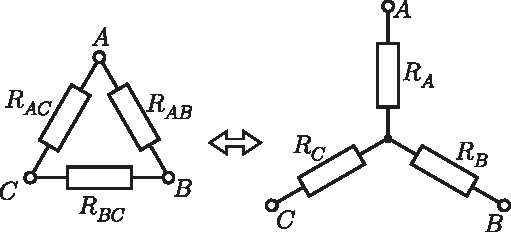
\includegraphics[width=8.2 cm]{ela5.pdf}	
	\centering
\end{figure}
\begin{question}[ela6][6cm]
	Leia joonisel kujutatud ahela takistus.
\end{question}

\textbf{Ideaalne ampermeeter ja voltmeeter.} Ideaalse ampermeetri sisetakistus on null ja ideaalse voltmeetri sisetakistus on lõpmatu.
\begin{question}[ela3][4.5 cm]
	Leia joonisel oleva ampermeetri näit.
\end{question}
\begin{question}[Lahtine 2015, N5][ela8][4.6 cm]
	Neli ühesugust takistit takistusega \( R \)	ning mõõteriistad on ühendatud nii nagu joonisel näidatud. Vooluallika
	pinge on \( U \).
	\begin{subquestion}
		\item Leia mõõteriistade näidud.
		\item Leia mõõteriistade näidud, kui vahetatakse ampermeetri ja voltmeetri asukohad.
	\end{subquestion}
\end{question}

\textbf{Superpositsiooniprintsiip.} Ohmi seadus ning Kirchhoffi seadused on lineaarsed, seetõttu vaid oomilisi takisteid ja elektromotoorjõu allikaid sisaldavas elektriahelas toimib \textit{superpositsiooniprintsiip} järgmisel kujul: resultatiivne voolutugevus läbi antud takisti on võrdne kõigi nende voolutugevuste algebralise summaga, mida indutseeriksid läbi selle takist kõik elektromotoorjõu allikad eraldi (st kõik teised elektromotoorjõu allikad lühistatakse).
\begin{question}[ela4][3.7cm]
	Joonisel toodud skeemis on tegemist ühesuguste takistitega takistustega $ R_1 = R_2 = R_3 = R_4 = R $ ning ühesuguste ideaalsete patareidega elektromotoorjõududega $ \mathcal{E}_1 = \mathcal{E}_2 = \mathcal{E} $. Leidke voolutugevused takistites (st $ I_1 $, $ I_2 $, $ I_3 $ ja $ I_4 $ avaldised suuruste $ R $ ja $ \mathcal{E} $ kaudu).
\end{question}

\textbf{Lõpmatud perioodilised ahelad.} Lõpmatutele perioodilistele ahelate uurimisel on kasulik ahela sarnasus iseendaga: esimese lüli eemaldamine ei muuda selle omadusi.
\begin{question}[ela7][9cm]
	Leia joonisel oleva ahela takistus.
\end{question}

\textbf{Lõpmatu perioodiline võre.} Superpositsiooniprintsiipi kasutades võib olla võimalik mittesümmeetriline probleem muuta sümmeetriliseks.
\begin{question}
	\label{lpv}
	Leia kahe naabersõlme A ja B vaheline takistus ruutvõres. Naabersõlmed on ühendatud traadijuppidega, mille takistus on \( R \).
\end{question}

\textbf{Negatiivne takistus.} Mõnikord on võimalik muuta probleem sümmeetriliseks kasutades fiktiivseid negatiivseid takistusi. \( R \) ja \( -R \) jadaühendus vastab null takistusele, rööpühenduses lõpmatule takistusele.
\begin{question}
	Lahendage ülesanne \ref{lpv} juhul, kui A ja B vaheline traadijupp on eemaldatud.
\end{question}

\section{Mittelineaarsed elemendid}
\textbf{Ideaalne diood.} \textit{Diood} on pooljuhtseadis, mis ühes suunas juhib voolu võrdlemisi hästi, vastassuunas peaaegu mitte. Dioodi nimetatakse ideaalseks, kui päripinge korral on selle takistus null ja vastupinge korral lõpmata suur. Veidi realistlikum (aga siiski idealiseeritud) dioodi tunnusjoone mudel on, kus diood avaneb täielikult teatud positiivse pinge \( U_d \) juures ja sellest madalamatel pingetel on täielikult suletud.
\begin{question}[ela9][\columnwidth]
	Mitu korda muutub joonisel toodud skeemis voolutugevus läbi pingeallika, kui viimase polaarsus muuta vastupidiseks?	Kõik takistid on võrdsed, dioodid ja elektromotoorjõuallikas on ideaalsed.
\end{question}

\textbf{Graafiline meetod.} Kui elektriahelas on elemente, mille voltamperkarakteristika \( I(U) \) pole lineaarne, siis on võimalik leida elemendist läbi mineva voolu graafiliselt. \( I(U) \)-sõltuvuse on võimalik ka avaldada Kirchhoffi seadustest, lihtsamatel juhtudel on see lineaarne seos \( U=U_0-IR \). Lahend(id) on kahe leitud joone, \( U_0-IR \) ja \( I(U) \), lõikepunkt(id).

\begin{question}[ela10][8.4cm]
	Kui suur on voolutugevus joonisel toodud ahelas? Dioodi voltamperkarakteristik on toodud juuresoleval graafikul.
\end{question}
\begin{question}[E-S 2003, P4][ela11][\columnwidth]
	Tunneldiood on hariliku dioodi sarnane pooljuhtseade, mida kirjeldagem pinge ja voolu vahelise tunnusjoone abil, vt graafikut. Skeemil on toodud lihtsaim tunneldioodil baseeruv võimendi. Leidke,
	mitu korda võimendatakse sisendisse antavat väikese amplituudiga
	signaale. \( R=10\ \Omega\), \( \mathcal{E}=0,25\ V \).
\end{question}

\end{document}